\renewcommand{\baselinestretch}{1.25}%
\begin{figure}[!t]%
  \centering
  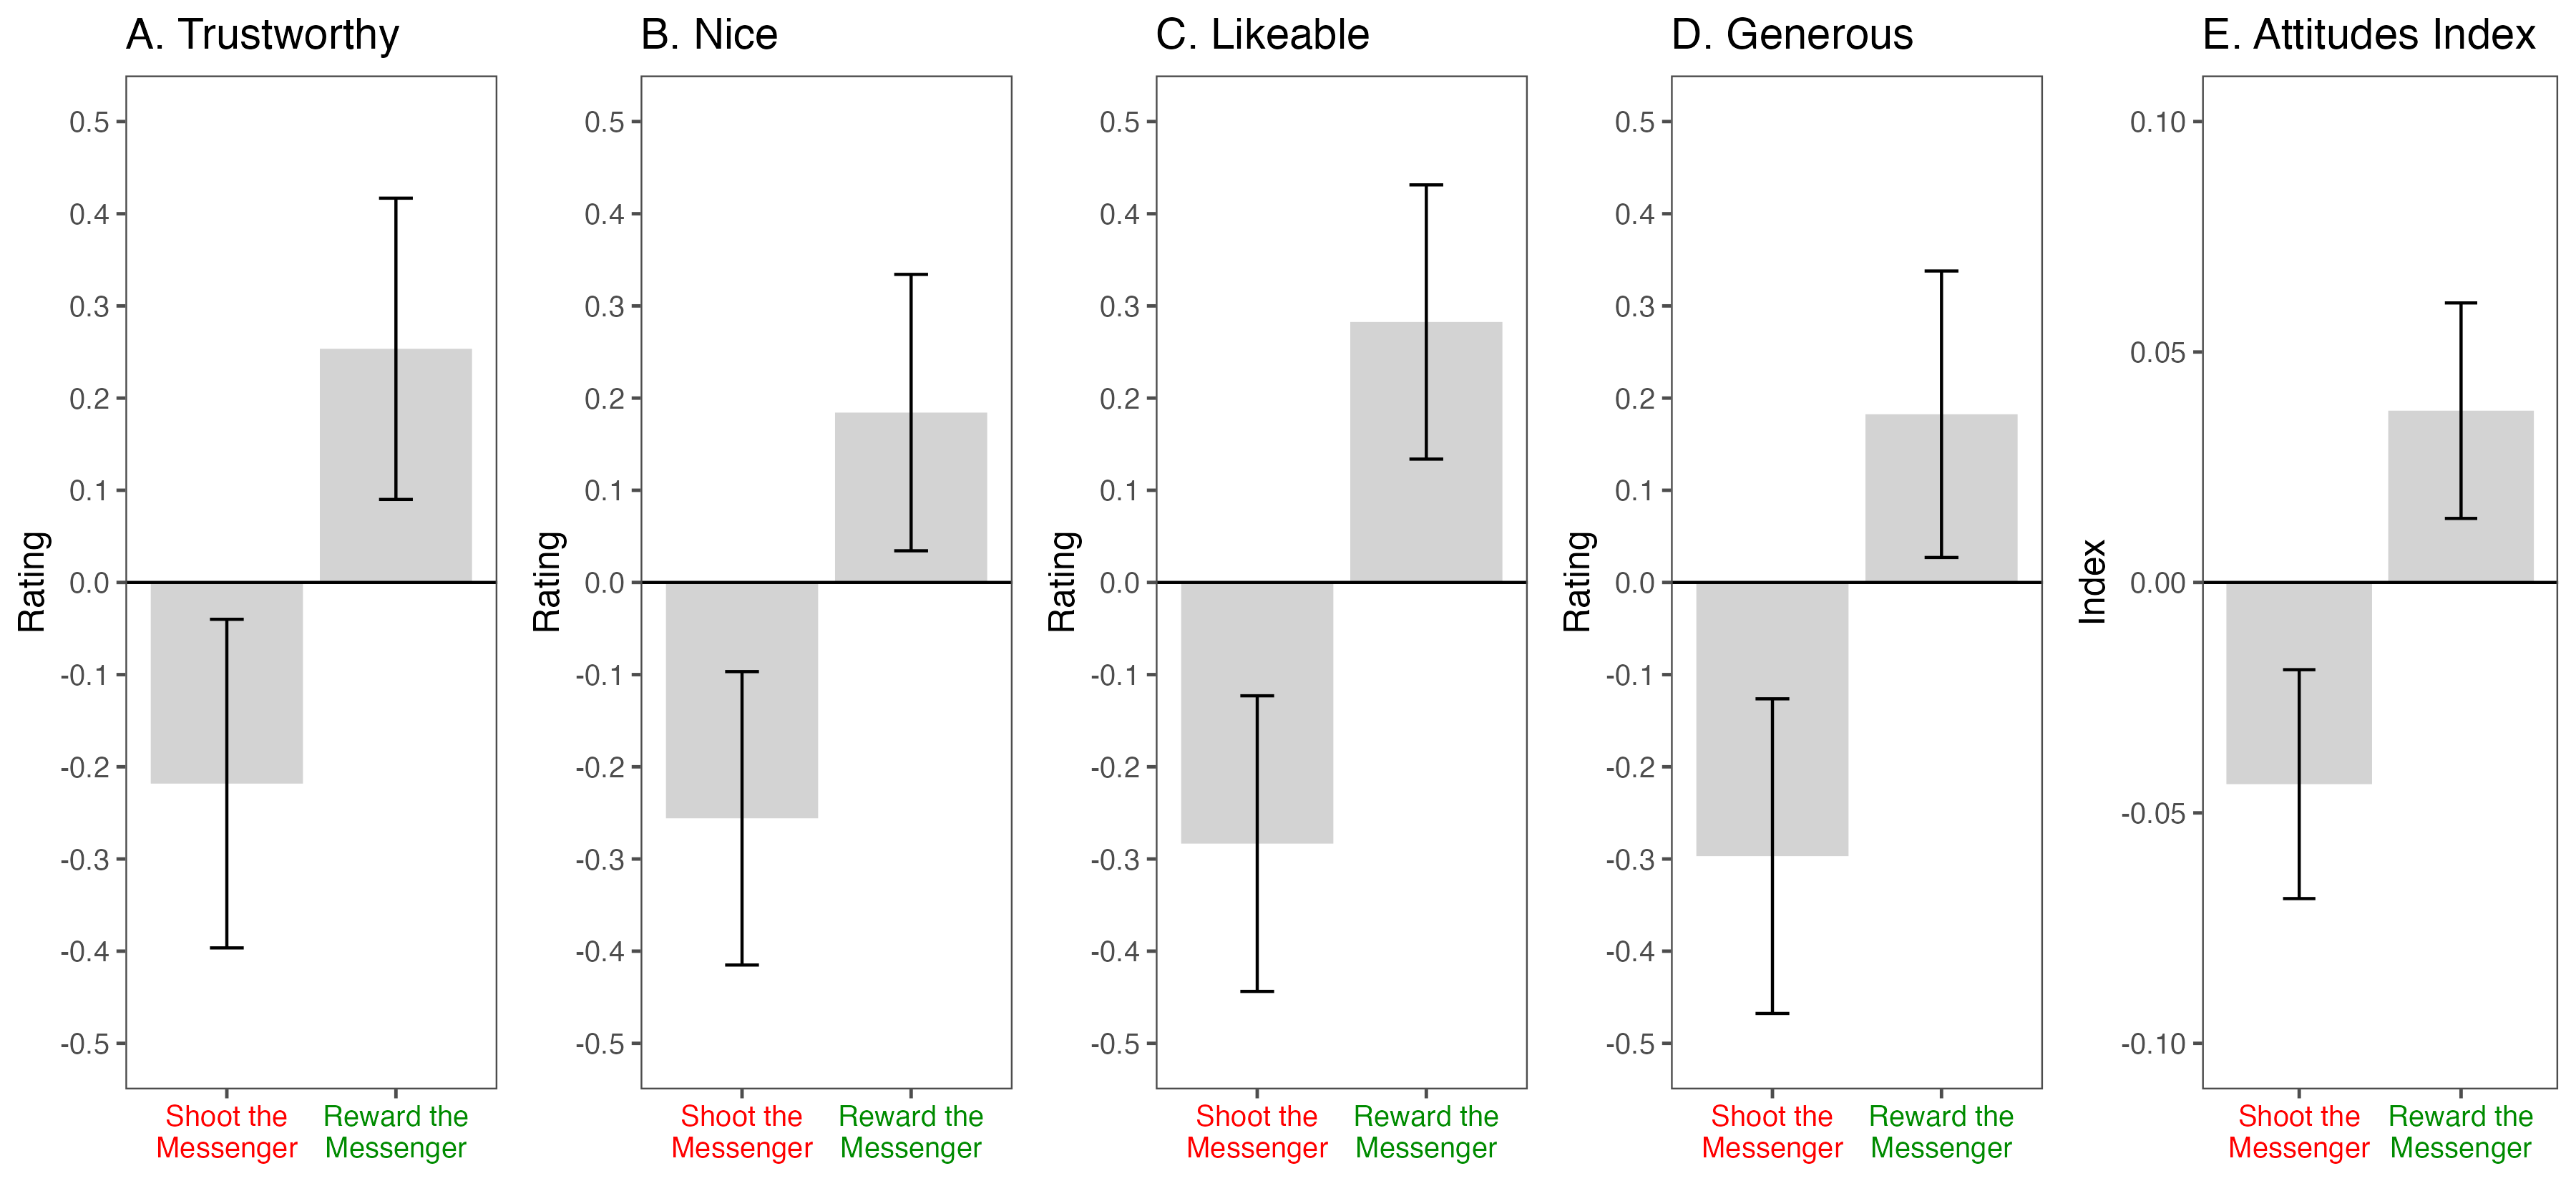
\includegraphics[width=1.0\textwidth]{figures/study1_attitude_list.png}
  \caption{Difference in the DVs of the attitude measures for messengers and non-messengers 
                                              by losing (STM) and winning (RTM), Study 1. 
  \textit{Note: OLS regression with robust standard errors, with error bars representing 95\% confidence intervals. The trustworthy (Panel A), nice (Panel B), likeable (Panel C), and generous (Panel D) dependent variables asks respondents to rate these messenger's characteristics on a 7-point Likert scale, where a score of 1 indicates that the messenger does not have that trait at all, while a score of 7 means that a trait describes the messenger extremely well.
    In the attitudes index (Panel E), the DV is calculated by averaging the ratings of the trustworthy, nice, likeable, and generous DVs to an index ranging from 0 to 1. The p-values of the test that $RTM = -STM$ are 0.77, 0.52, 0.99, 0.33, and 0.71, respectively, for each facet and index. The p-values of messenger bias are 0.00, 0.00, 0.00, 0.00, and 0.00, respectively, for each facet and the index.}}
  \label{fig:attitude_list}
\end{figure}%
\renewcommand{\baselinestretch}{1.67}%
